% ============================================================================ EXPLORE
\section{Exploring the Design Space}\label{sec:explore}

Exploration works at two levels. At the converter level the synthesis is repeated over the
regulator count and the topology (Section~\ref{sec:dse}, Fig.~\ref{fig:dse}): the optimum moves
to 76 cells with a two-branch topology, and a sweep with the topology held fixed misses it
because its feasible range ends at 52 cells. At the package level, every input without a single
defensible value is varied on the production mesh and the full chain is rerun, so that each
ranking of Section~\ref{sec:compare} is reported together with the decisions that can change
it. Fig.~\ref{fig:robust} summarizes \NvariantRuns{} such runs for the embedded and
package-backside pair at S0: for each decision and each ranking, whether the ranking is
preserved, withdrawn (the gap falls within twice its uncertainty) or reversed.

\begin{figure}[!t]
\centering
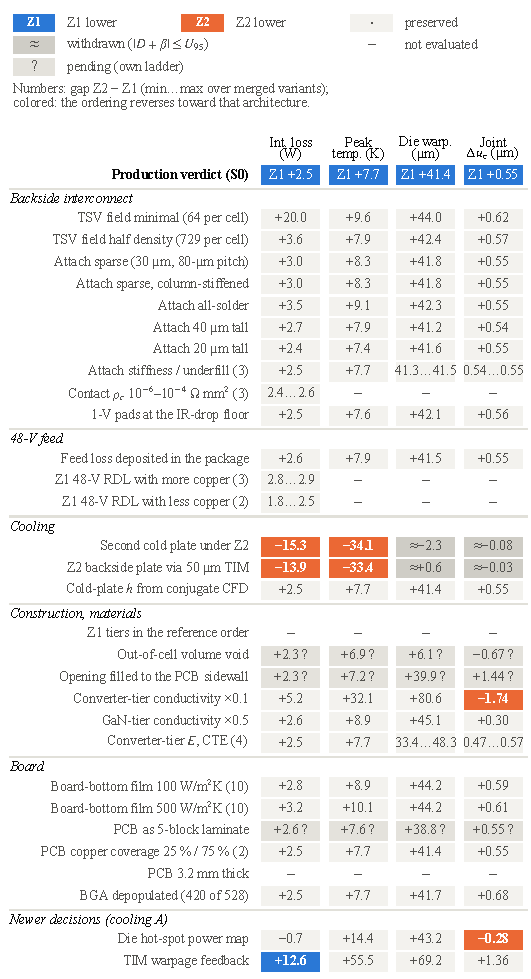
\includegraphics[width=\columnwidth]{fig9_robustness_map.pdf}
\caption{Ranking-robustness map, Z1 against Z2 at S0. Rows: package decisions varied on the
production mesh, grouped by the design choice they represent (merged rows give the number of
runs); columns: the rankings. Each cell shows whether the production ranking is preserved,
withdrawn (gap within twice its uncertainty) or reversed, with the architecture it then
favors.}
\label{fig:robust}
\end{figure}

% TODO(data): which decisions preserve / withdraw / reverse each ranking:
%  - tier order (z1_tier_reference): +x K, +y W -- realizability and electrothermal coupled
%  - backside cooling (z2_cooled): reverses the thermal and mechanical rankings?
%  - TSV provisioning (tsv_min), attach density (attach_sparse): electrical ranking
%  - out-of-cell construction (f2_void): mechanical ranking
%  - board boundary (board_hbot100/500): joint temperatures, calibration flags
%  - cooling model form (icepak_equivalent): peak temperature
